\section{Estrutura}
A estrutura no ramo da engenharia é a área na qual utiliza de cálculos estruturais para dar forma a um objeto predefinido, determinando seus limites, materiais, estabilidade, dinâmica, vibração entre outros fatores. O objetivo da estrutura em um projeto é dar forma como um todo, levando em consideração cálculos estruturais analíticos ou mesmo simulações computacionais que facilitam na obtenção dos resultados. Além disso, com a parte estrutural pode-se integrar os demais subsistemas necessários.
Os principais fatores levados em consideração na análise estrutural de um projeto é se os materiais escolhidos são os melhores, mas com o melhor preço, se ele suportará as cargas aplicadas, não apresentando deformações plásticas e se o mesmo não sofrerá danos em decorrência de vibrações.
\subsection{Materiais}
Para a estrutura da estufa automatizada é necessário um material que seja resistente às cargas que serão aplicadas, ao mesmo tempo que seja viável financeiramente. Foram escolhidos dois metais para a estrutura interna, são eles o alumínio e o aço, materiais com resistências variadas e de relativa fácil usinagem, mas que suportam sem problema algum a massa de componentes tais como os motores, sensores e placas a serem acrescentadas no interior. As cantoneiras de aço, principal material estrutural do projeto, podem vir conforme duas normas técnicas brasileiras de aplicação do aço:
\begin{itemize}
	\item Norma NBR 6591: Norma padrão para aço carbono com costura, para peças que tem como uso final a utilização em estrutura e indústrias em geral. Nessa norma não há exigências de propriedades mecânicas ou acabamento, mas há a exigência da definição das propriedades químicas.
	
	\item Norma NBR 8261: Norma padrão para tubos de aço carbono, com costura opcional e formação à frio, no lugar da formação à quente, própria para peças destinadas à utilização em estruturas soldadas, parafusadas ou rebitadas.
\end{itemize}
Nessa última norma, as cantoneiras de aço podem ainda vir em composições diferentes, com maior ou menor grau de carbono, e que diferem no tratamento químico recebido e em suas propriedades mecânicas \cite{tubonasa}.
Como se trata de um protótipo e a principal característica a ser cuidada é a sustentação da estufa, as propriedades que foram levados em consideração para referencial teórico foram as tensões conforme as propriedades médias de um aço com 0,2\% de carbono, que é aproximadamente a composição do metalon \cite{callister2002wd}:
\begin{itemize}
	\item Massa volumétrica: 7860 kg/m$^{3}$ (ou 7,86 $g/cm^{3}$)
	\item Coeficiente de expansão térmica: 11,7 $10^{-6}$ ($^{\circ}C)^{-1}$
	\item Condutividade térmica:52,9 W/m-K
	\item Calor específico: 486 J/kg-K
	\item Resistividade elétrica: 1,6 10$^{-7}\Omega$m
	\item Módulo de elasticidade (Módulo de Young) Longitudinal: 210GPa
	\item Módulo de elasticidade (Módulo de Young) transversal:80 GPa
	\item Coeficiente de Poisson: 0,3
	\item Limite de escoamento: 210 MPa
	\item Limite de resistência à tração: 380 MPa
	\item Alongamento: 25\%
\end{itemize}

A figura \ref{fig:propriedade_material} representa as propriedades do material utilizado para as simulações feitas no Software de modelagem 3D CATIA V5R19. Nota-se a extrema semelhança com os dados coletados pela referência, o que garante a veracidade dos resultados obtidos em simulação em relação ao projeto real:
\begin{figure}[H]
	\centering
	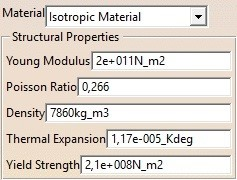
\includegraphics[width=5cm]{figuras/propriedade_material.jpg}
	\caption{Propriedades do material simulado}
	\label{fig:propriedade_material}
\end{figure}
O acabamento da estufa tanto interno como externo está sendo desenvolvido para que cumpra com o papel de revestimento térmico, levando em consideração estética, vedação e viabilidade financeira. Os materiais utilizados para tal finalidade são isopor, chapa de PVC, espuma expansiva e silicone.
\subsubsection{Resistência dos materiais}

É pelo estudo das mecânicas dos materiais que o engenheiro consegue dimensionar uma estrutura. Saber o tamanho de uma barra, qual diâmetro ela necessita ter para suportar um dado peso sem haver perdas de materiais, ou em qual ponto pode ocorrer uma ruptura. 
Dentre os esforços mais sentidos pela estrutura da estufa estão os de tensão normal e flexão. Com isso, para saber se tais materiais propostos são resistentes às cargas que serão aplicadas, algumas teorias devem ser estudadas.
TENSÃO NORMAL: Uma força aplicada em uma determinada área está exercendo uma tensão, e quando tal força e área são perpendiculares é chamada de tensão normal, como mostra a figura \ref{fig:tensao_normal}. 
\begin{figure}[H]
	\centering
	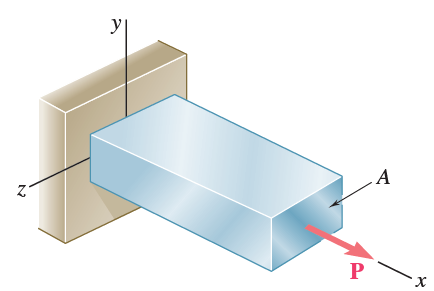
\includegraphics[width=8cm]{figuras/tensao_normal.png}
	\caption{Tensão normal sobre uma barra prismática}
	\label{fig:tensao_normal}
\end{figure}

FLEXÃO: Quando uma força paralela ao eixo longitudinal é aplicada a um elemento estrutural alongado e o mesmo sofre uma deformação é caracterizado como flexão. Tem como aspecto uma deformação na forma de arco, figura \ref{fig:flexao_pura}.
\begin{figure}[H]
	\centering
	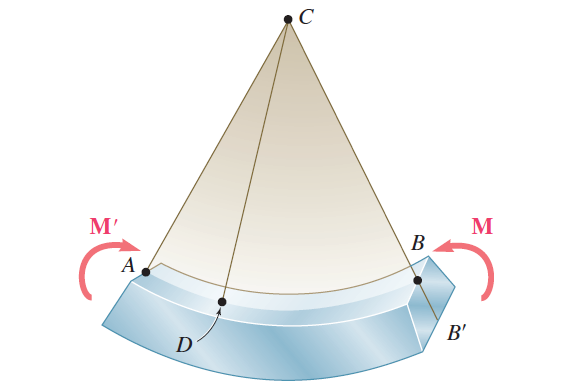
\includegraphics[width=8cm]{figuras/flexao_pura.png}
	\caption{Flexão pura sobre uma barra prismática}
	\label{fig:flexao_pura}
\end{figure}

\subsubsection{Vibrações}

Em vários sistemas é muito comum ocorrer o fenômeno da vibração. Ela pode causar desgastes prematuros de superfícies em contato e dependendo da sua frequência pode até mesmo colapsar toda a estrutura, assim o estudo da vibração é necessária para que funcione de maneira desejada. A figura \ref{fig:esquema_excitacao} apresenta um esquema básico de vibração causado pela base do sistema.
\begin{figure}[H]
	\centering
	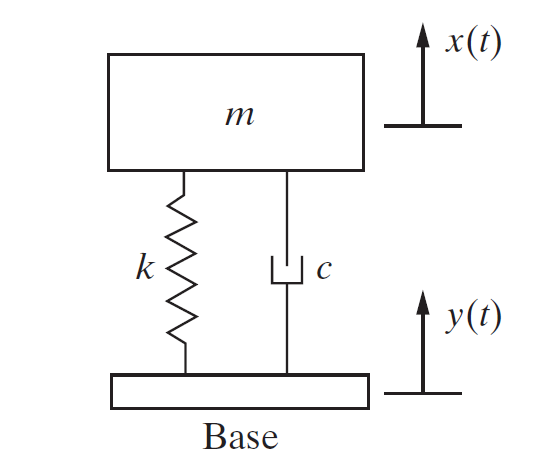
\includegraphics[width=8cm]{figuras/esquema_excitacao.png}
	\caption{Esquema de uma excitação pela base}
	\label{fig:esquema_excitacao}
\end{figure}

A análise de vibração, como o próprio nome diz, visa analisar as variações nas vibrações das máquinas. Ao avaliar alguma alteração nela, é possível prever problemas que podem vir a ocorrer no desempenho dos equipamentos, além de determinar quais peças que necessitam de manutenção. Outra função dessa análise é para que os especialistas consigam melhorar as condições de trabalho das máquinas. Portanto, ela é de fundamental importância dentro do conceito de manutenção preditiva, já que avalia de forma eficiente as condições dos equipamentos e, consequentemente, evita defeitos e falhas inesperadas \cite{nobrega2014}.

Sensores são colocados em pontos estratégicos das máquinas, transformando as vibrações em sinais elétricos, que por sua vez são encaminhados para aparelhos registradores de vibrações. Os dados coletados serão analisados por um profissional capacitado, que avaliará se há algum problema ou não naquele equipamento. Para a implementação da análise de vibração, primeiro é avaliada qual máquina deve ser monitorada. Logo em seguida, é feito um cadastramento dela no sistema de monitoramento, definindo as faixas de medição, parâmetros utilizados e a frequência de coleta dos dados. Em um terceiro momento é definida uma rota para a coleta de dados de acordo com as máquinas e equipamentos definidos e há um acompanhamento nos dados coletados. Depois é emitido um relatório com as condições das máquinas e equipamentos, mostrando potenciais defeitos e recomendações para corrigi-los \cite{nobrega2014}.
Ao realizar este procedimento, há uma redução nos custos de manutenção, já que é possível prever quando é necessário a intervenção de manutenção, além do já citado prolongamento da vida útil dos componentes. Some isso ao aumento da eficiência das intervenções de manutenção, aumento da disponibilidade dos equipamentos, ampliação da confiabilidade operacional e redução no curso de conversão.


A manutenção preditiva baseia-se na avaliação do estado da máquina com inspeções de rotina. Com isso, elimina-se o desperdício de peças, diminui-se os estoques associados, aumenta a eficiência nos reparos, reduz ou elimina problemas e aumenta a disponibilidade das máquinas. Portanto, ela é excelente na questão de custo-benefício, já que dependendo da indústria, os custos com a manutenção representam até 30\% dos investimentos da empresa \cite{zuniga2011}.
\subsubsection{Transferência de calor}

Um dos principais requisitos para a construção da estufa é que a temperatura interna seja controlada, pois é muito importante controlar a mesma para que as plantas tenham um crescimento saudável. Esse trabalho será realizado tanto pelos materiais isolantes como pelo cooler de refrigeração. Tal ciência é estudada através da transferência de calor. Este fenômeno dita que dois ou mais corpos próximos ou em um mesmo ambiente tendem a trocar calor até que todos entrem em equilíbrio térmico.
\subsubsubsection{Condução}

A condução é uma forma de transferência onde uma partícula mais energética transfere a sua energia para uma menos energética, figura \ref{fig:conducao_termica}. Os níveis de condução variam principalmente de acordo com o material, alguns transferem a sua energia mais rapidamente do que outros, como por exemplos os metais, na qual são considerados bons condutores térmicos. Para o caso da estufa utilizou-se o isopor junto com o PVC para fazer esse trabalho de evitar condução, já que os dois são materiais que possuem uma baixa condutividade térmica.
\begin{figure}[H]
	\centering
	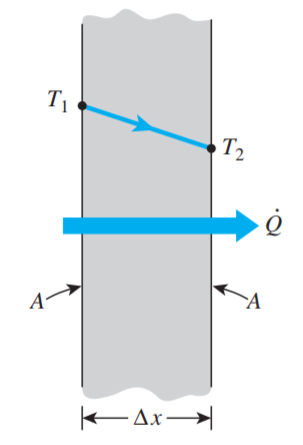
\includegraphics[width=10cm]{figuras/conducao_termica.png}
	\caption{Condução térmica em um sólido}
	\label{fig:conducao_termica}
\end{figure}

\subsubsubsection{Convecção}

Este modo de transferência se dá através do movimento combinado de um fluido por uma superfície sólida, figura \ref{fig:conveccao_termica}. O movimento da água dentro de um cano cria a convecção, gerando uma transferência de calor em consequência do fluxo. A dinâmica do ar dentro e fora da estufa provocará esse fenômeno físico, agindo nas paredes de isopor, PVC e madeira. Para que esse efeito não influencie demais na temperatura ambiente os materiais devem ser bons isolantes.
\begin{figure}[H]
	\centering
	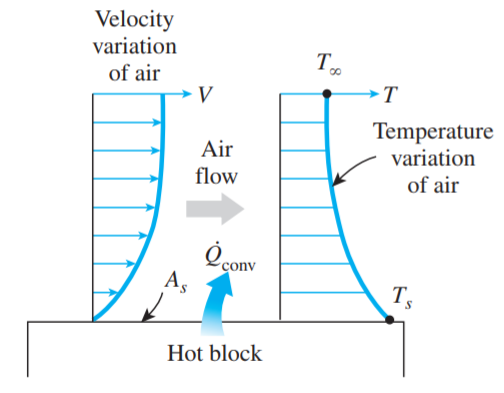
\includegraphics[width=10cm]{figuras/conveccao_termica.png}
	\caption{Convecção térmica do ar sobre um sólido}
	\label{fig:conveccao_termica}
\end{figure}

\subsubsubsection{Radiação}

A radiação é a energia emitida pela matéria na forma de ondas eletromagnéticas, figura \ref{fig:radiacao_termica}. A energia emitida pelo Sol e sentida aqui na Terra como forma de calor é dada pela transferência da radiação. Objetos criados pelo homem, como as lâmpadas, também emitem energia pela radiação. Com isso, haverá um possível aumento da energia interna da estufa ao longo do tempo em consequência da utilização de lâmpadas, mas que poderá ser facilmente corrigida pelo resfriamento do ar através dos coolers.
\begin{figure}[H]
	\centering
	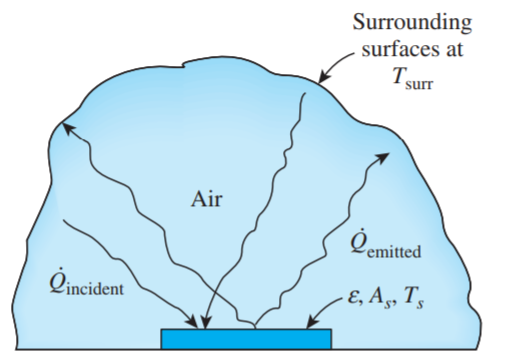
\includegraphics[width=10cm]{figuras/radiacao_termica.png}
	\caption{Transferência de calor pela radiação entre superfícies vizinhas }
	\label{fig:radiacao_termica}
\end{figure}